\begin{figure}[h]
  \centering
  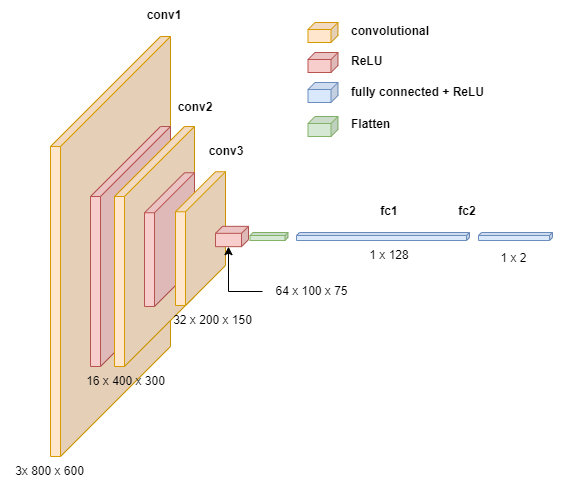
\includegraphics[width=0.5\textwidth]{assets/early-work/cnn-diagram.png}
  \caption{One of the best models for the agent reaching task}\label{fig:cnn-5050}
\end{figure}


\begin{figure}[htbp]
  \centering
  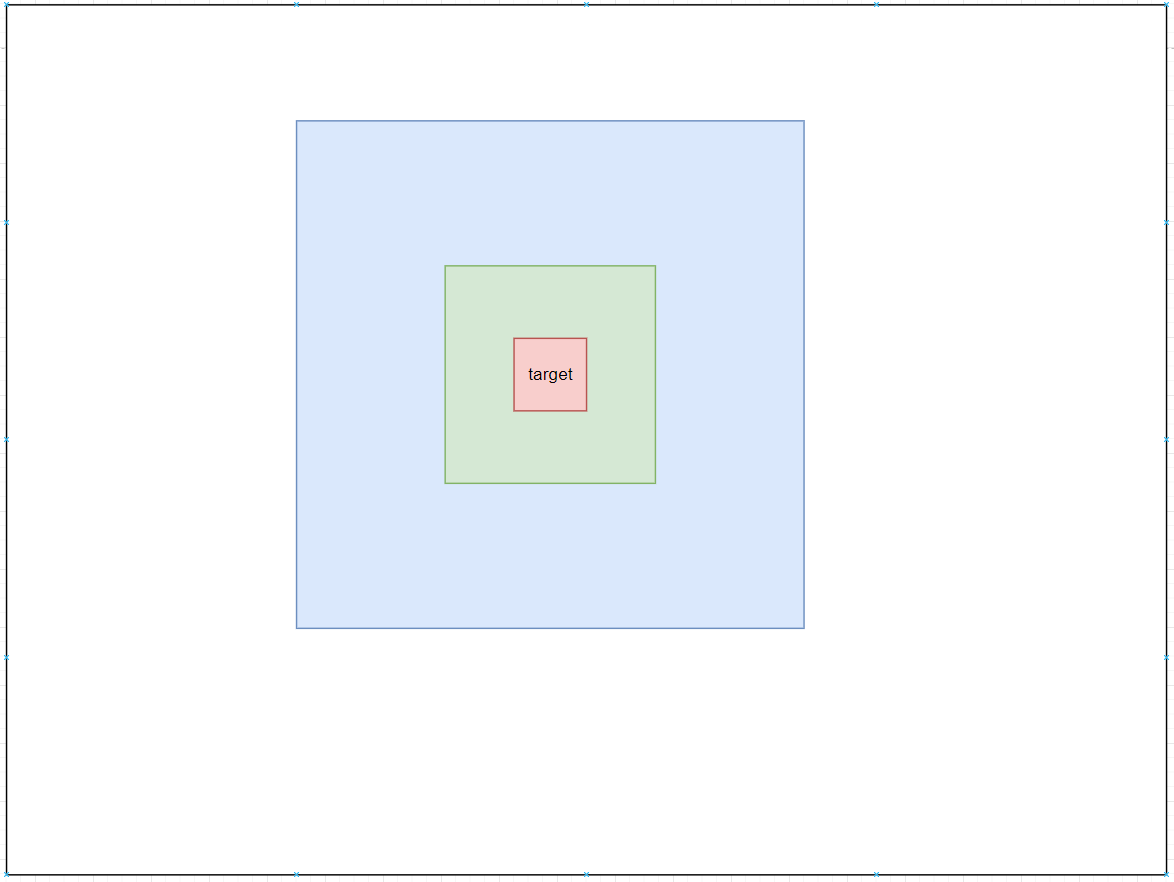
\includegraphics[width=0.5\textwidth]{assets/early-work/regions.png}
  \caption{Illustration of phases around the target, 0 would be green, 1 would be blue and 2 would be the rest of the canvas in this example. }\label{fig:phase-regions}
\end{figure}


\begin{figure}[htbp]
  \centering
  \begin{subfigure}{0.45\textwidth}
      \centering
      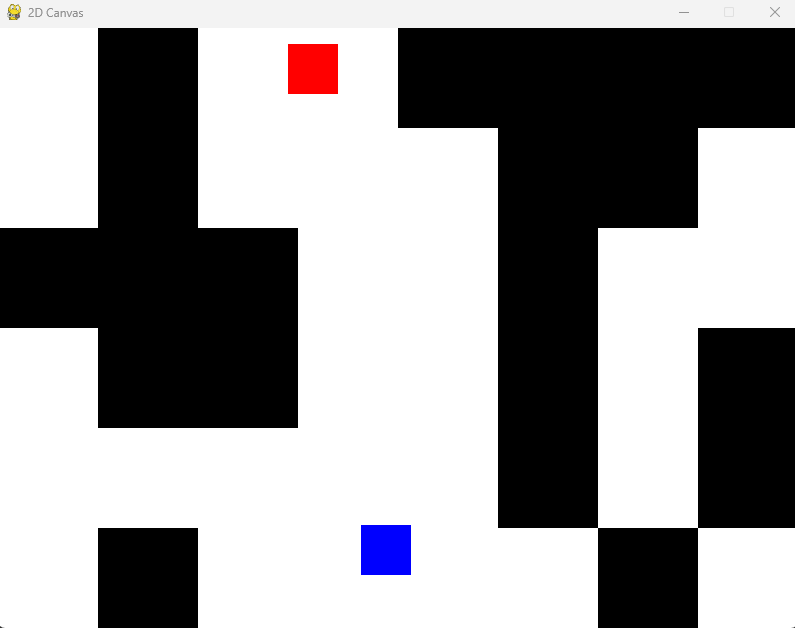
\includegraphics[width=0.6\linewidth]{assets/early-work/obs-gen1.png}
      \caption{Example 1}
  \end{subfigure}%
  \hfill
  \begin{subfigure}{0.45\textwidth}
      \centering
      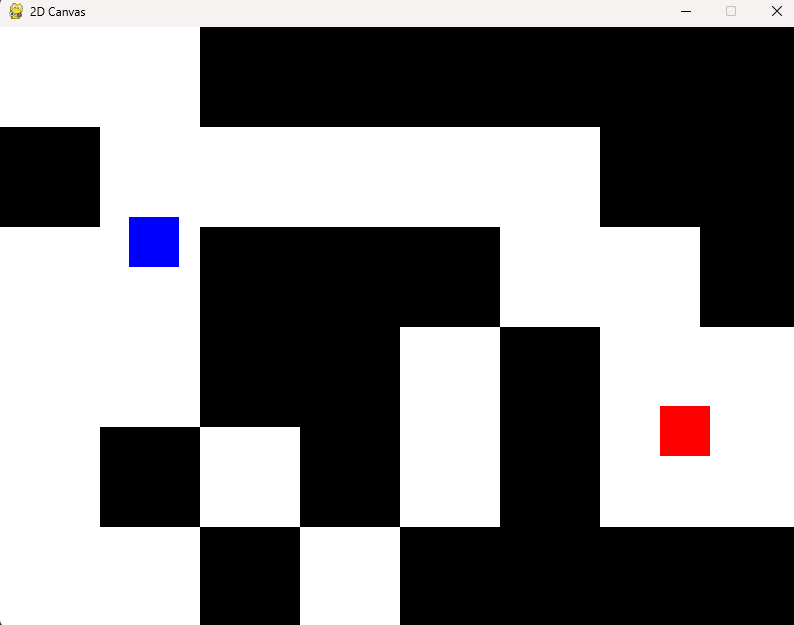
\includegraphics[width=0.6\linewidth]{assets/early-work/obs-gen2.png}
      \caption{Example 2}
  \end{subfigure}

  \vspace{0.5cm}

  \begin{subfigure}{0.45\textwidth}
      \centering
      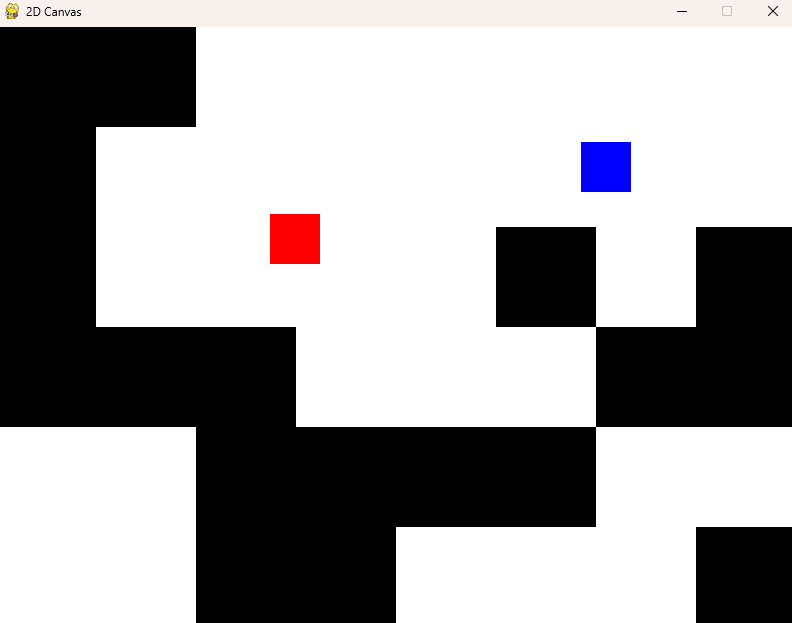
\includegraphics[width=0.6\linewidth]{assets/early-work/obs-gen3.png}
      \caption{Example 3}
  \end{subfigure}%
  \hfill
  \begin{subfigure}{0.45\textwidth}
      \centering
      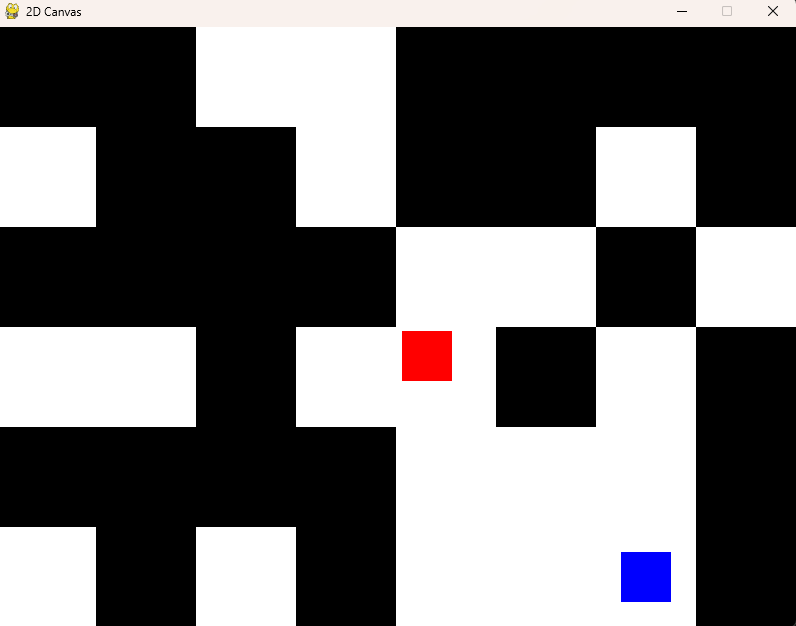
\includegraphics[width=0.6\linewidth]{assets/early-work/obs-gen4.png}
      \caption{Example 4}
  \end{subfigure}
  \caption{The 2 by 2 grid of some example obstacle generations}\label{fig:obs-gen}
\end{figure}




\begin{figure}[htpb] % htpb allows all placement
  \centering
  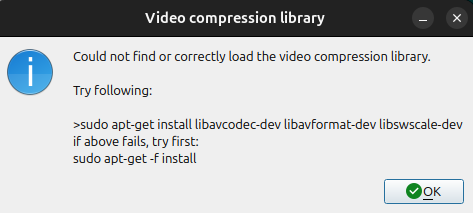
\includegraphics[scale=0.3]{assets/early-work/missing-libs.png}
  \caption{}\label{fig:missing-libs}
\end{figure}

\begin{listing}[H]
  \begin{minted}[fontsize=\small, bgcolor=gray!10, linenos]{python}

  obs_config = ObservationConfig().set_all(True) 
  enabled_config = CameraConfig(
    rgb=True, depth=False, mask=False, point_cloud=False, image_size=(64, 64)
    render_mode=RenderMode.OPENGL,
  )
  disabled_config = CameraConfig(
    rgb=False, depth=False, mask=False, render_mode=RenderMode.OPENGL)

  obs_config.wrist_camera = enabled_config ## example: enabling a cam/sensor
  obs_config.front_camera = disabled_config

  env = Environment(
    action_mode = MoveArmThenGripper(
      arm_action_mode=JointVelocity(), 
      gripper_action_mode=Discrete()
    ),
    dataset_root = '' if live_demos else 'PATH/TO/YOUR/DATASET',
    obs_config = obs_config, headless = False
  )
  env.launch() ## start the simulator
  \end{minted}
  \caption{Standardised environment launching}\label{lst:env-setup}
\end{listing}